\documentclass{article}
\usepackage{graphicx}
\usepackage{float}
\usepackage{epstopdf}

\begin{document} 
\begin{center}
{\bf \Large  Homework 7} \\
\end{center}
Chien-Pin Chen\\
cchen144\\

The HW6 figure shows a robot moving left. While moving, it measures each second ($\Delta T$ = 1s) the distance from the obstacle behind it (the corner) and the obstacle
in front of it (the wall). In this scenario, we consider the corner as the reference
point, i.e., with the coordinate 0. As shown in class, in order to simultaneously
estimate the robot position and the position of the wall, we use the state vector
$\underline{x}$ with the following three components: $x_1$ is the robot position measured from
the corner, $x_2$ is the robot velocity with the positive direction towards the wall
and $x_3$ is the wall position measured from the corner. The measurement $y_1$ is
the distance from the robot to the corner and $y_2$ is the distance from the robot
to the wall. A linear model describing this scenario is
\begin{equation}
  \underline{x}(k+1)=\left[ 
  \begin{array}{ccc}
     1 & 1 & 0  \\
     0 & 1 & 0  \\
     0 & 0 & 1 
  \end{array}
   \right] \underline{x}(k)+ \left[
     \begin{array}{c}
     0   \\
     0.1   \\
     0
  \end{array}
   \right] w(k)
\end{equation}
where the Gaussian random variable w(k) has zero mean and variance 1. The
observation model is
\begin{equation}
 \underline{y}(k) =\left[
     \begin{array}{ccc}
     1 & 0 &  0  \\
     -1 & 0 & 1   
  \end{array}
   \right] \underline{x}(k)+\underline{\theta}(k)
\end{equation}
where the covariance matrix of Gaussian measurement noise $\underbar{$\theta$}$ 
is $diag(10, 10)$. All variables in the above equations are expressed in $cm$ and $cm=s$.

The course webpage (HW6) provides you the sequence of the measurements
$y_1$ and $y_2$ recorded for $k = 1, 2,...$ in the fille roboMes.mat. The data are
organized so that $y(1, k)$ denotes the measurement $y_1(k)$ and $y(2, k)$ 
denotes the measurement $y_2(k)$, where $k=1,2,3....$. 

Design the Kalman smoother that takes the measurement sequences and
produces the estimation sequences of the robot position, its velocity and the
distance between the wall and the corner given all available data. \\

a) Plot on the same diagram the result of the forward Kalman filter and
RTS backward iterations for {\bf the robot position}.

b) Plot on the same diagram the result of the forward Kalman filter and
RTS backward iterations for {\bf the robot velocity}.

d) Plot on the same diagram the result of the forward Kalman filter and
RTS backward iterations for {\bf the wall position}.

e) For the robot position, compare the variance resulting from the Kalman
filter and the variance resulting from the smoother.

Comment your results and trends in data. {\bf Note:} Please keep in mind that
you can use your Kalman filter code from HW6 with a slight modification, i.e.,
after removing 0.8 in the equation defining the velocity. Choose your initial
condition for $x_1(0)$ and $x_3(0)$, as well as corresponding variances the 
same way you did for the Kalman filter in HW6. {\bf However, for $x_2(0)$ use the 
initial condition $0.2$ or $1.6$ and the variance $1$.}

\noindent \textbf{ANS:}\\
For forward Kalman filter, I could use equations from homework 5 with slightly modify:
\begin{eqnarray}
x_{k + 1}  = \Phi x_k  + \Gamma w_k \\
y_k  = {\rm H}x_k  + v_k 
\end{eqnarray}
then, for computing in homework 7, I could set:
\begin{eqnarray}
\Phi  = \left[ {\begin{array}{*{20}c}
   1 & 1 & 0  \\
   0 & 0 & 0  \\
   0 & 0 & 1  \\
\end{array}} \right],{\rm{ }}\Gamma  = \left[ {\begin{array}{*{20}c}
   0  \\
   {0.1}  \\
   0  \\
\end{array}} \right],{\rm{ and }}Q = {\mathop{\rm var}} (w(k)) = 1\\
{\rm H} = \left[ {\begin{array}{*{20}c}
   {\begin{array}{*{20}c}
   1 & 0 & 0  \\
\end{array}}  \\
   {\begin{array}{*{20}c}
   { - 1} & 0 & 1  \\
\end{array}}  \\
\end{array}} \right],{\rm{ and }}R = {\mathop{\rm var}} (\theta (k)) = \left[ {\begin{array}{*{20}c}
   {10} & 0  \\
   0 & {10}  \\
\end{array}} \right]
\end{eqnarray}
Now, I could use the same steps in homework 5 for computing forward Kalman filter in MATLAB.
After forward Kalman filter, I get the sequence of the result of $\underline{\hat{x}}_k$ and $\underline{\hat{P}}_k$, and 
I could use the last elements in both sequence as initial value (condition) to do Kalman smoother with RTS algorithms:
\begin{eqnarray}
\underline{\hat{x}}_{k\left| N \right.}  = \underline{\hat{x}}_k ( + ) + A_k (\underline{\hat{x}}_{k + 1\left| N \right.}  - \underline{\hat{x}}_{k + 1} ( - )), \; \underline{\hat{x}}_{N\left| N \right.}  = \underline{\hat{x}}_N ( + )\\
\underline{A}_k  = \underline{P}_k ( + )\Phi _k^T \underline{P}_{k + 1}^{ - 1} ( - )\\
\underline{P}_{k\left| N \right.}  = \underline{P}_k ( + ) + \underline{A}_k (\underline{P}_{k + 1\left| N \right.}  - \underline{P}_{k + 1} ( - ))\underline{A}_k^T , \;  \underline{P}_{N\left| N \right.}  = \underline{P}_N ( + )
\end{eqnarray} 
And, after computing Kalman smoother and forward Kalman filter, I could plot the results as below:\\
\textbf{(a)} The diagram of results of the robot position.\\
From the below diagram, the result of Kalman smoother is smooth and each data point is not diverse a lot from the real data. 

\begin{figure}[H]
\begin{center}
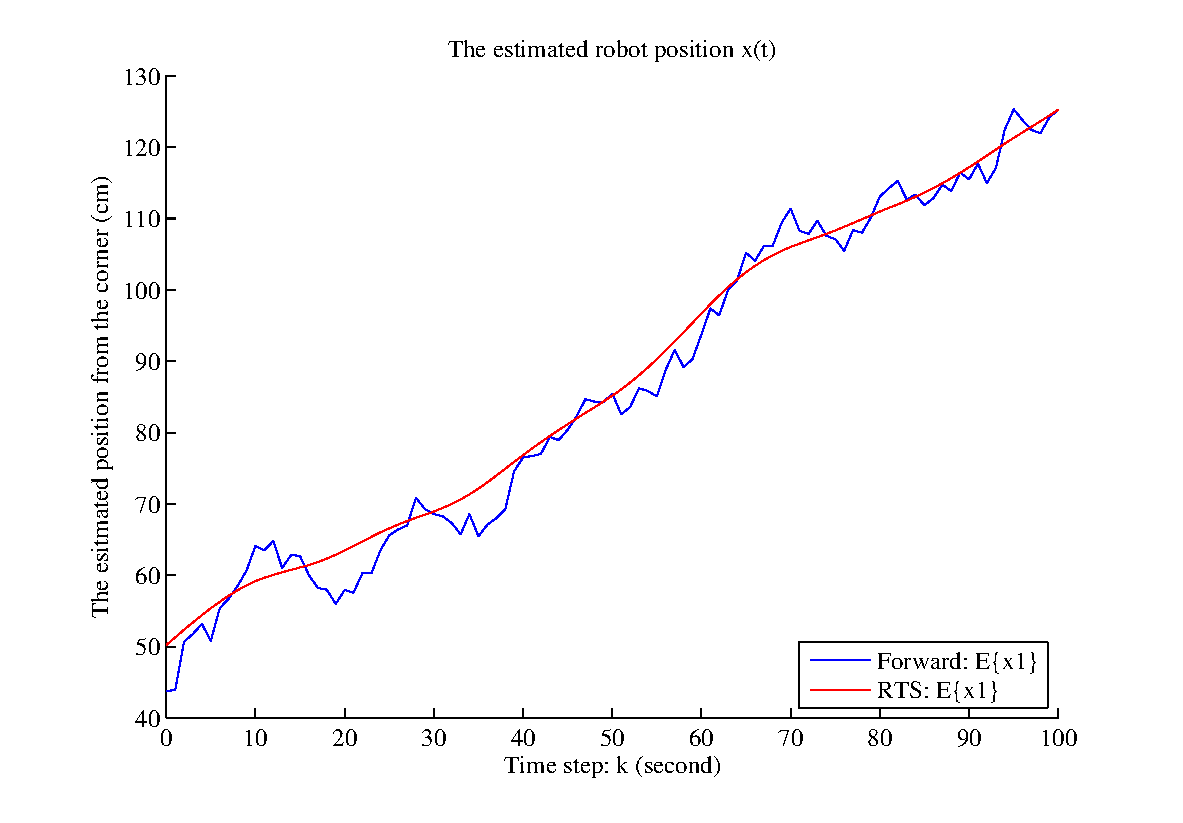
\includegraphics[scale=0.6]{hw7_x1.eps}
\end{center}
\end{figure}

\textbf{(b)}The diagram of results of the robot velocity.\\
The result of velocity is also smooth, but it has more obviously turning curve. And, as indicated in "Applied Optimal Estimation",
the result of smoother tends to lag (from backward) the measurement data whenever it has large changing curve.

\begin{figure}[H]
\begin{center}
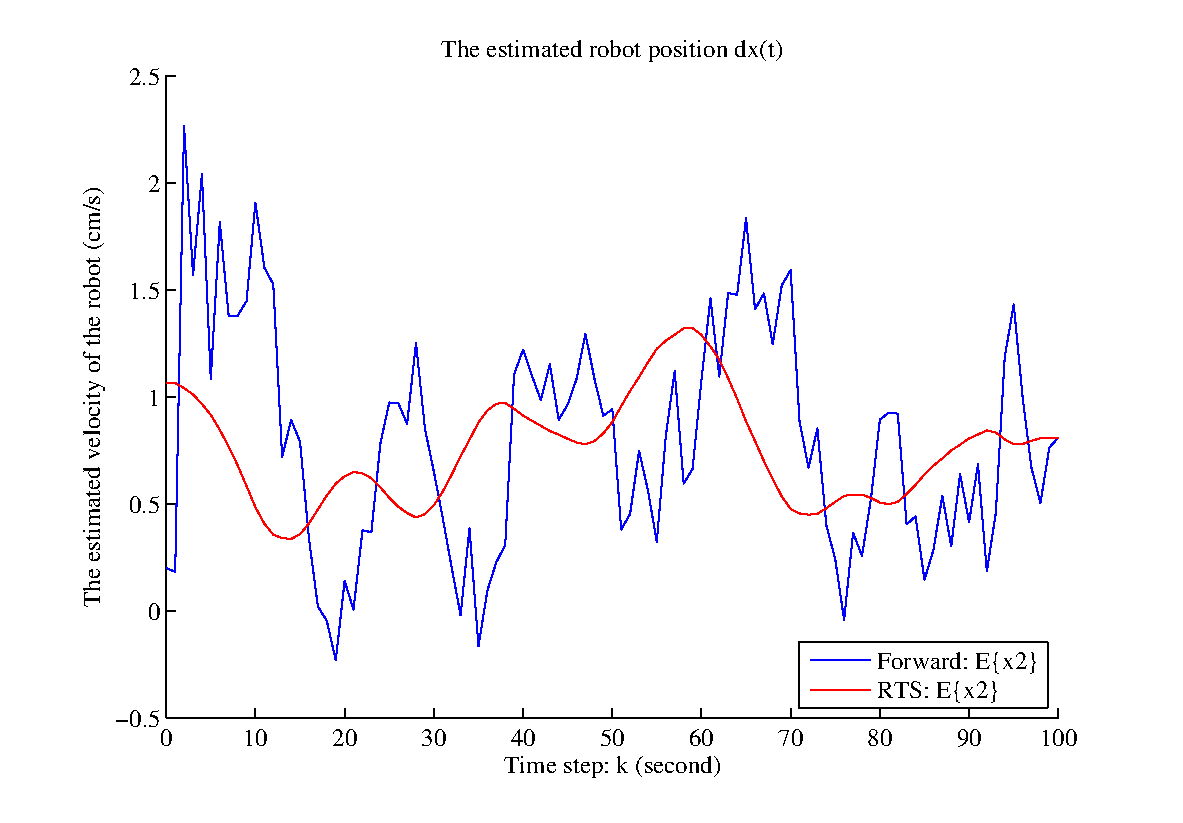
\includegraphics[scale=0.6]{hw7_x2.eps}
\end{center}
\end{figure}

\noindent \textbf{(d)} The diagram of results of the wall position.\\
The result of wall position, after Kalman smoother, is fixed even when the measurement data are fluctuated.

\begin{figure}[H]
\begin{center}
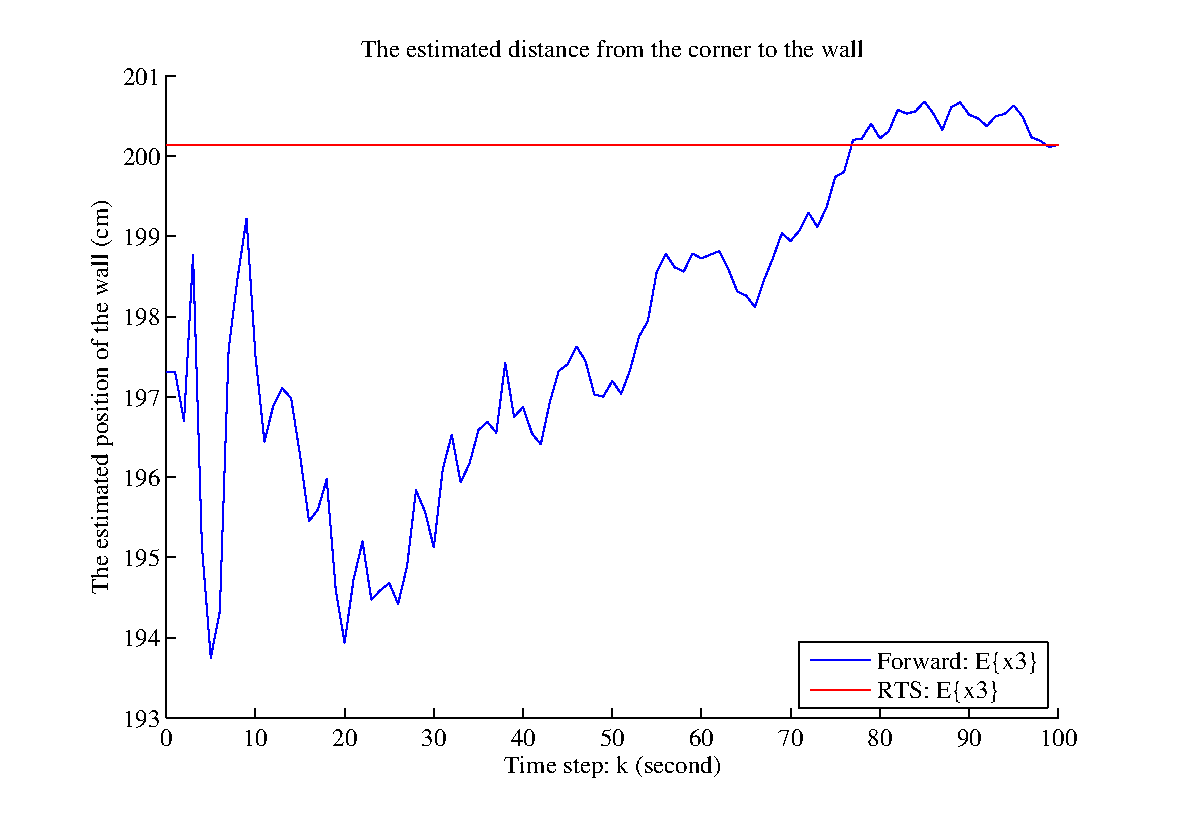
\includegraphics[scale=0.6]{hw7_x3.eps}
\end{center}
\end{figure}

\noindent \textbf{(e)} The diagram of results of the variance of the robot position\\
From the below results, the variance from forward Kalman filter start to decrease and converge after 30 second.
And, for RTS backward smoother, the variance start to decrease from 100 second and converge after 90 second.
Although the variance of the backward after 10 second start to increase, it is still smaller than the variance of forward 
in the same time interval.

\begin{figure}[H]
\begin{center}
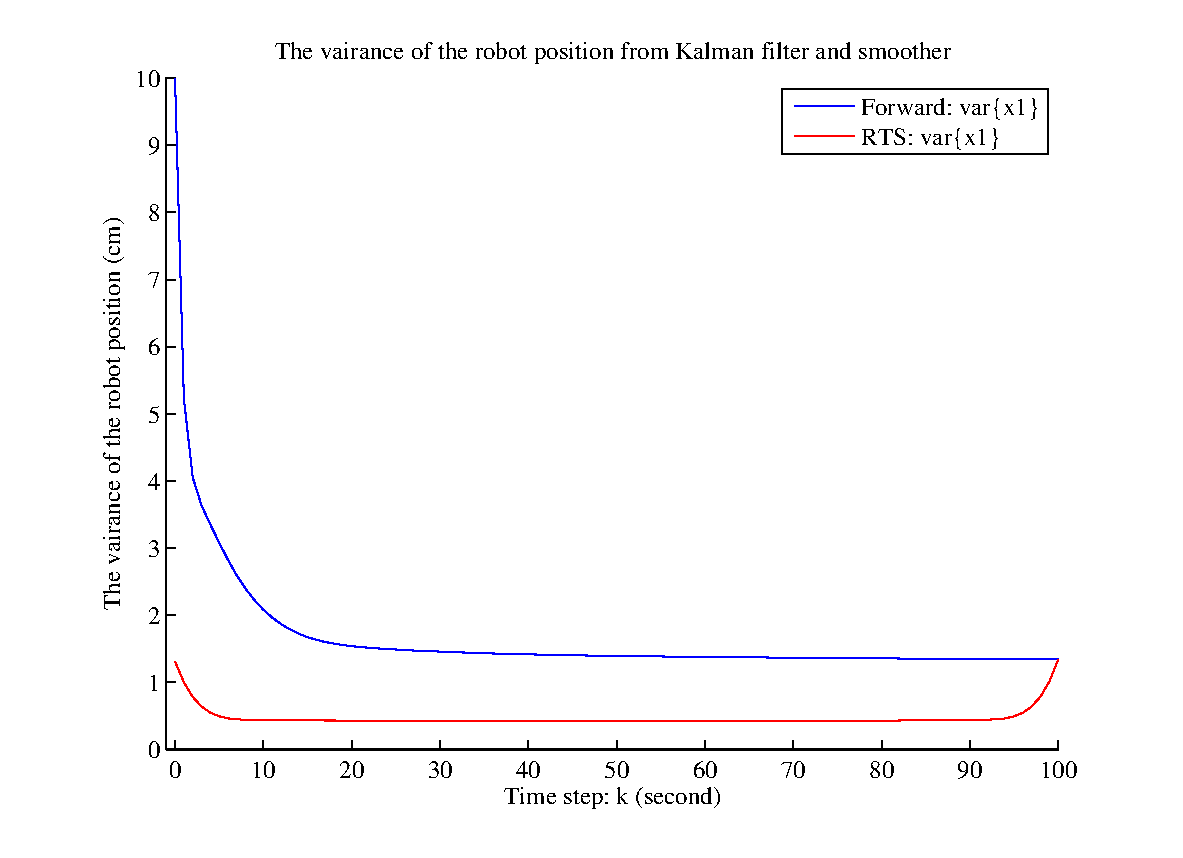
\includegraphics[scale=0.6]{hw7_varx13.eps}
\end{center}
\end{figure}

\end{document}
